\documentclass[10pt]{beamer}

\usepackage[utf8x]{inputenc}
\usepackage[OT4]{fontenc}

\usepackage[polish]{babel}

\setbeamertemplate{navigation symbols}{}

\usetheme[bullet=circle,
          titleline=true,
          pageofpages=z,
          alternativetitlepage=true]{Torino}

\usepackage{ragged2e}
\usepackage{hyphenat}
\usepackage{hyperref}
\usepackage{booktabs}
\usepackage{listings}
\usepackage{multibib}

\usepackage{tikz}
\usepackage{pgfplots}

\usetikzlibrary{arrows}
\usetikzlibrary{automata}
\usetikzlibrary{backgrounds}
\usetikzlibrary{decorations}

\usepackage{amsmath}
\usepackage{amsfonts}
\usepackage{amsthm}

\usepackage{highlight/pythonhighlight}

\title{SymPy --- czyli matematyka w Pythonie}
\author{Mateusz Paprocki \texttt{<mattpap@gmail.com>}}
\institute{Wrocław University of Technology \\ University of Nevada, Reno}
\date{\today}

\newenvironment{jblock}[1]{
    \begin{block}{#1}\justifying\nohyphens
}{
    \end{block}
}

\setbeamercovered{transparent}

\begin{document}

\begin{frame}[plain,t]
    \maketitle
\end{frame}

\begin{frame}
    \frametitle{Plan prezentacji}
    \framesubtitle{}

    \begin{itemize}
        \item Matematyka w Pythonie
        \item Wprowadzenie do SymPy
        \item Architektura systemu
        \item Przykłady zastosowań
        \item Sesja interaktywna
        \item Plany na przyszłość
    \end{itemize}
\end{frame}

\begin{frame}[fragile]
    \frametitle{Matematyka w Pythonie}
    \framesubtitle{}

    \begin{itemize}
        \item Python:
            \begin{itemize}
                \item \verb+__add__+, \verb+__sub__+, \verb+__mul__+, \verb+__div__+, \ldots
            \end{itemize}
        \pause
        \item \texttt{math}:
            \begin{itemize}
                \item biblioteka numeryczna
                \item jedynie funkcje rzeczywiste
                \item logarytmy i funkcja wykładnicza
                \item funkcje trygonometryczne i hiperboliczne
            \end{itemize}
        \pause
        \item NumPy \& SciPy
            \begin{itemize}
                \item biblioteki numeryczne
                \item działania na macierzach
                \item funkcje rzeczywiste i zespolone
                \item optymalizacja, interpolacja, \ldots
            \end{itemize}
        \pause
        \item Swiginac, Pynac, Sage, \ldots, SymPy
    \end{itemize}
\end{frame}

\begin{frame}[fragile]
    \frametitle{Dlaczego SymPy?}

    Istnieje wiele systemów matematycznych:
    \begin{itemize}
        \item Systemy \structure{komercyjne}:
            \begin{itemize}
                \item Mathematica, Maple, Magma, \ldots
            \end{itemize}
        \item Systemy \structure{Open Source}:
            \begin{itemize}
                \item AXIOM, GiNaC, Maxima, PARI, Sage, Singular, Yacas, \ldots
            \end{itemize}
    \end{itemize}
    \pause
    {\color{red} Problemy:}
    \begin{itemize}
        \item wszystkie \structure{wymyślają} swój własny \structure{język programowania}
            \begin{itemize}
                \item musimy się takiego języka nauczyć (często bywają uciążliwe)
                \item podział na jądro systemu oraz bibliotekę matematyczną
                \item \structure{wyjątki}: GiNaC and Sage
            \end{itemize}
        \pause
        \item wszystkie wymagają kompilacji
            \begin{itemize}
                \item niekorzystne w użyciu interaktywnym
            \end{itemize}
    \end{itemize}
\end{frame}

\begin{frame}[fragile]
    \frametitle{Co to jest SymPy?}
    \framesubtitle{}

    SymPy jest to \structure{biblioteka} pisana w \structure{Pythonie} do wykonywania:
    \begin{itemize}
        \pause
        \item obliczeń symbolicznych
            \begin{itemize}
                \item np. wyznaczanie pochodnych, całek, sum, granic, szeregów
            \end{itemize}
        \pause
        \item obliczeń algebraicznych
            \begin{itemize}
                \item np. wyznaczanie izomorfizmów ciał algebraicznych
            \end{itemize}
        \pause
        \item obliczeń numerycznych
            \begin{itemize}
                \item np. rozwiązywanie równań nieliniowych
            \end{itemize}
    \end{itemize}
\end{frame}

\begin{frame}[fragile]
    \frametitle{Przykładowa sesja z SymPy}
    \framesubtitle{}

    \begin{itemize}
        \item import \texttt{sympy} i definicja symboli
            \begin{python}
>>> from sympy import *
>>> var('x,y')
            \end{python}
        \pause
        \item całkowanie oraz upraszczanie wyrażeń
            \begin{python}
>>> f = (x - tan(x)) / tan(x)**2 + tan(x)

>>> integrate(f, x)
log(1 + tan(x)**2)/2 - x/tan(x) - x**2/2

>>> ratsimp(_.diff(x)) == f
True
            \end{python}
    \pause
        \item rozkład wielomianów na czynniki
            \begin{python}
>>> factor(x**2 + y**2, extension=I)
(x - I*y)*(x + I*y)
            \end{python}
        \pause
        \item wyznaczanie wartości funkcji specjalnych
            \begin{python}
>>> gamma(pi).evalf(n=30)
2.28803779534003241795958890906
            \end{python}
    \end{itemize}
\end{frame}

\begin{frame}
    \frametitle{Założenia projektu}
    \framesubtitle{}

    \begin{itemize}
        \item biblioteka pisana w Pythonie
            \begin{itemize}
                \item bez nowego środowiska, języka, \ldots
                \item działa od razu na dowolnej platformie
                \item moduły nie--Pythonowe mogą być opcjonalne
            \end{itemize}
            \pause
        \item prostota architektury
            \begin{itemize}
                \item relatywnie mała baza kodu źródłowego
                \item łatwość w rozbudowie na dowolnym poziomie
            \end{itemize}
            \pause
        \item szeroka funkcjonalność
            \begin{itemize}
                \item obsługa najważniejszych działów matematyki
                \item wspieranie zaawansowanych metod i algorytmów
            \end{itemize}
            \pause
        \item optymalizacja wydajności w Cythonie
            \begin{itemize}
                \item opcjonalnie, jako dodatek do wersji interpretowanej
            \end{itemize}
            \pause
        \item liberalna licencja: BSD
            \begin{itemize}
                \item duża swoboda w użytkowaniu SymPy
            \end{itemize}
    \end{itemize}
\end{frame}

\begin{frame}[fragile]
    \frametitle{SymPy w liczbach}

    \begin{itemize}
        \item 2006--teraz
        \pause
        \item 100 autorów
        \item 150 tysięcy linii kodu
            \begin{itemize}
                \item 500 klas
                \item 8000 funkcji
            \end{itemize}
        \item 17 tysięcy testów
            \begin{itemize}
                \item czas wykonania: 8 minut (Atom 1.6)
            \end{itemize}
        \pause
        \item 11 prezentacji na konferencjach i warsztatach
        \item 16 projektów w Google Summer of Code
            \begin{itemize}
                \item oraz Google Highly Open Participation Contest
            \end{itemize}
        \item jedna praca dyplomowa
    \end{itemize}
\end{frame}

\begin{frame}[fragile]
    \frametitle{Informacje kontaktowe}

    \begin{itemize}
        \item Strona główna projektu:
            \begin{itemize}
                \item \texttt{www.sympy.org}
            \end{itemize}
        \item Strony dodatkowe:
            \begin{itemize}
                \item \texttt{docs.sympy.org}
                \item \texttt{wiki.sympy.org}
                \item \texttt{live.sympy.org}
            \end{itemize}
        \pause
        \item Lista mailingowa:
            \begin{itemize}
                \item \texttt{sympy@googlegroups.com}
            \end{itemize}
        \item Kanał IRC:
            \begin{itemize}
                \item \texttt{\#sympy} na FreeNode
            \end{itemize}
        \pause
        \item Repozytorium \texttt{git}:
        \begin{verbatim}
        git clone git://github.com/sympy/sympy.git
        \end{verbatim}
    \end{itemize}
\end{frame}

\begin{frame}[fragile]
    \frametitle{Organizacja pracy}
    \framesubtitle{}

    \begin{itemize}
        \item korzystamy z systemu SCM \texttt{git}
        \pause
        \item jedno główne repozytorium (GitHub)
            \begin{itemize}
                \item tylko jedna gałąź --- \texttt{master}
            \end{itemize}
        \item każdy twórca ma własny ``fork'' na GitHubie
            \begin{itemize}
                \item zazwyczaj wiele gałęzi
            \end{itemize}
        \pause
        \item żeby zacząć pracę z jedną z gałęzi:
            {\small
            \begin{verbatim}
git remote add github git://github.com/mattpap/sympy-polys.git
git fetch github
git branch --track polys11 github/polys11
            \end{verbatim}}
        \pause
        \item korzystamy z mechanizmu ``pull request'' do łączenia gałęzi
        \pause
        \item testy zawsze muszą wykonywać się poprawnie
            \begin{itemize}
                \item używamy buildbotów do testowania różnych konfiguracji
            \end{itemize}
    \end{itemize}
\end{frame}

\begin{frame}
    \frametitle{Moja rola w projekcie}
    \framesubtitle{}

    \begin{itemize}
        \item początek współpracy w marcu 2007 roku
            \begin{itemize}
                \item kilka prostych poprawek i rozszerzeń
            \end{itemize}
        \pause
        \item następnie Google Summer of Code 2007
            \begin{itemize}
                \item algorytmy rozwiązywania równań rekurencyjnych
                \item algorytmy sumowania nieoznaczonego i oznaczonego
            \end{itemize}
        \pause
        \item no i tak już zostało:
            \begin{itemize}
                \item algorytmy całkowania symbolicznego
                \item struktury algebraiczne, wielomiany
                \item upraszczanie wyrażeń algebraicznych, \ldots
            \end{itemize}
        \pause
        \item poza tym:
            \begin{itemize}
                \item Google Summer of Code 2009, 2010 mentor (PSU, PSF)
                \item EuroSciPy 2009, 2010; py4science (UC Berkeley)
                \item praca dyplomowa
            \end{itemize}
    \end{itemize}
\end{frame}

\begin{frame}
    \frametitle{Moduły SymPy}
    \framesubtitle{}

    \begin{columns}
        \begin{column}[l]{0.3\textwidth}
            \begin{itemize}
                \item assumptions
                \item concrete
                \item core
                \item functions
                \item galgebra
                \item geometry
                \item integrals
                \item interactive
            \end{itemize}
        \end{column}
        \pause
        \begin{column}[l]{0.3\textwidth}
            \begin{itemize}
                \item logic
                \item matrices
                \item mpmath
                \item ntheory
                \item parsing
                \item physics
                \item plotting
                \item polys
            \end{itemize}
        \end{column}
        \pause
        \begin{column}[l]{0.3\textwidth}
            \begin{itemize}
                \item printing
                \item series
                \item simplify
                \item solvers
                \item statistics
                \item tensor
                \item thirdparty
                \item utilities
            \end{itemize}
        \end{column}
    \end{columns}
\end{frame}

\begin{frame}
    \frametitle{Zastosowania SymPy}
    \framesubtitle{}

    \begin{itemize}
        \item rozwiązywanie problemów \structure{matematycznych}
            \begin{itemize}
                \item np. nauczanie matematyki
                \item Dlaczego?
                    \begin{itemize}
                        \item łatwy do nauczenia język programowania
                        \item użytkownik ma dostęp do wszystkich algorytmów
                    \end{itemize}
                \item Przykład: $k$--kolorowanie grafów
            \end{itemize}
        \pause
        \item \structure{osadzanie} SymPy w innych programach
            \begin{itemize}
                \item np. generacja kodu na podstawie wyrażeń matematycznych
                \item Dlaczego?
                    \begin{itemize}
                        \item mała biblioteka bez żadnych zależności
                        \item nie wymaga kompilacji, instalacji, konfiguracji
                    \end{itemize}
                \item Przykład: generowanie kodu C
            \end{itemize}
    \end{itemize}
\end{frame}

\begin{frame}
    \frametitle{$k$--kolorowanie grafów (1)}

    \begin{columns}
        \begin{column}[l]{0.4\textwidth}
            \begin{center}
                \includegraphics<1->[scale=0.6]{images/graph-nocolor.pdf}
            \end{center}
        \end{column}
        \begin{column}[r]{0.4\textwidth}
            \begin{center}
                \includegraphics<2->[scale=0.6]{images/graph-color.pdf}
            \end{center}
        \end{column}
    \end{columns}
\end{frame}

\begin{frame}
    \frametitle{$k$--kolorowanie grafów (2)}

    Dany jest $\mathcal{G}(V, E)$. Wprowadzamy dwa układy równań wielomianowych:
    \begin{itemize}
        \item<2-> $I_k$ --- dozwolone jest przypisanie jednego z $k$ kolorów do wierzchołka $x_i$
            \begin{equation*}
                I_k = \{ x_i^k - 1 : i \in V \}
            \end{equation*}
        \item<3-> $I_{\mathcal{G}}$ --- przyległe wierzchołki muszą mieć przypisane różne kolory
            \begin{equation*}
                I_{\mathcal{G}} = \{ x_{i}^{k-1} + x_{i}^{k-2} x_{j} + \ldots + x_{i} x_{j}^{k-2} + x_{j}^{k-1} : (i, j) \in E \}
            \end{equation*}
    \end{itemize}
    \onslide<4->{
        Następnie rozwiązujemy $I_k \cup I_{\mathcal{G}}$ metodą baz Gr\"{o}bnera.
    }
\end{frame}

\begin{frame}
    \frametitle{$k$--kolorowanie grafów (3)}

    \begin{columns}
        \begin{column}[l]{0.4\textwidth}
            \begin{align*}
                \{& \structure{x_{1}} + x_{11} + x_{12},              \\
                  & \structure{x_{2}} - x_{11},                       \\
                  & \structure{x_{3}} - x_{12},                       \\
                  & \structure{x_{4}} - x_{12},                       \\
                  & \structure{x_{5}} + x_{11} + x_{12},              \\
                  & \structure{x_{6}} - x_{11},                       \\
                  & \structure{x_{7}} - x_{12},                       \\
                  & \structure{x_{8}} + x_{11} + x_{12},              \\
                  & \structure{x_{9}} - x_{11},                       \\
                  & \structure{x_{10}} + x_{11} + x_{12},             \\
                  & \structure{x_{11}}^2 + x_{11} x_{12} + x_{12}^2,  \\
                  & \structure{x_{12}}^3 - 1 \}
            \end{align*}
        \end{column}
        \begin{column}[r]{0.4\textwidth}
            \begin{center}
                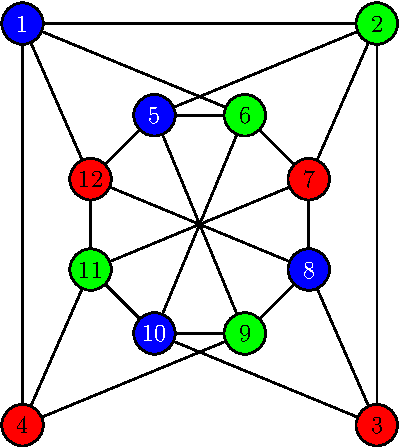
\includegraphics[scale=0.6]{images/graph-color.pdf}
            \end{center}
        \end{column}
    \end{columns}
\end{frame}

\begin{frame}[fragile]
    \frametitle{$k$--kolorowanie grafów (4)}

    Rozwiązanie problemu \structure{$3$--kolorowania} w SymPy:
    \begin{python}
In [1]: V = range(1, 12+1)
In [2]: E = [(1,2),(2,3),(1,4),(1,6),(1,12),(2,5),(2,7),
(3,8),(3,10),(4,11),(4,9),(5,6),(6,7),(7,8),(8,9),(9,10),
(10,11),(11,12),(5,12),(5,9),(6,10),(7,11),(8,12)]

In [3]: X = [ Symbol('x' + str(i)) for i in V ]
In [4]: E = [ (X[i-1], X[j-1]) for i, j in E ]

In [5]: I3 = [ x**3 - 1 for x in X ]
In [6]: Ig = [ x**2 + x*y + y**2 for x, y in E ]

In [7]: G = groebner(I3 + Ig, X, order='lex')

In [8]: G != [1]
Out[8]: True
    \end{python}
\end{frame}

\begin{frame}[fragile]
    \frametitle{$k$--kolorowanie grafów (5)}

    \begin{figure}
        \begin{center}
            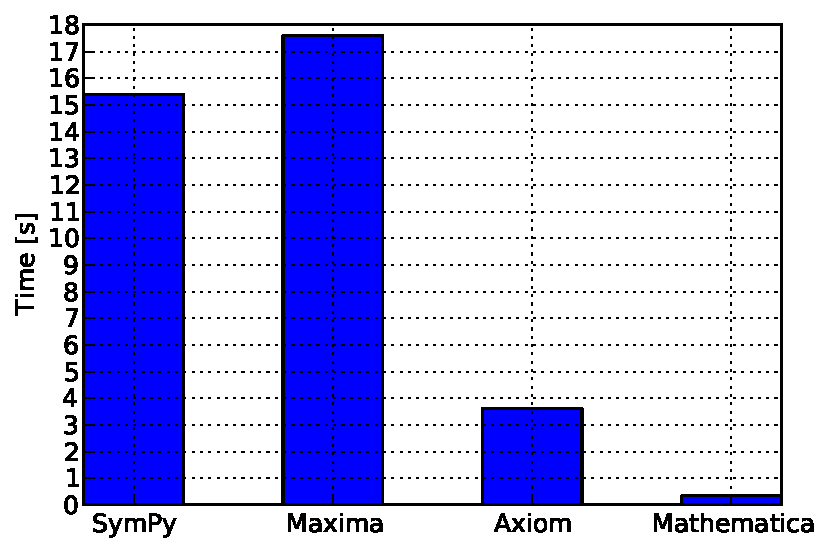
\includegraphics[scale=0.55]{images/groebner-time-compare.pdf}
        \end{center}
        \caption{Średni czas obliczania $3$--kolorowania dla grafu $\mathcal{G}(V, E)$.}
    \end{figure}
\end{frame}

\begin{frame}[fragile]
    \frametitle{Generowanie kodu C (1)}

    Sformułowanie problemu:
    \begin{itemize}
        \item transformacja wyrażeń do postaci \structure{Hornera}
        \item generacja odpowiadającego im kodu w \structure{języku C}
            \begin{itemize}
                \item np. dla celów szybkiego wyznaczenia wartości dla wielu punktów
            \end{itemize}
        \item przyjmijmy, że nie chcemy/nie możemy skorzystać z funkcji \texttt{pow()}
    \end{itemize}
    \vskip+0.5cm
    \pause
    Jak możemy rozwiązać tak sformułowany problem?
    \begin{itemize}
        \item używamy funkcji \texttt{horner()} do transformacji wyrażeń
        \item definiujemy nową \structure{drukarkę} do wygenerowania kodu
    \end{itemize}
\end{frame}

\begin{frame}[fragile]
    \frametitle{Generowanie kodu C (2)}

    Definiujemy nową \structure{drukarkę} dla sformułowanego problemu:
    \begin{python}
from sympy.printing import StrPrinter

class CPrinter(StrPrinter):
    """Print Lambda as C function and unroll Pow. """

    counter = 0

    def _print_Lambda(self, expr):
        self.counter += 1

        return """long _f%i(long %s) {\n  return (%s);\n}""" % \
            (self.counter, expr.args[0], self.doprint(expr.args[1]))

    def _print_Pow(self, expr):
        if expr.exp.is_Integer:
            return '*'.join([str(expr.base)]*int(expr.exp))
        else:
            return StrPrinter._print_Pow(self, expr)
    \end{python}
\end{frame}

\begin{frame}[fragile]
    \frametitle{Generowanie kodu C (3)}

    Chcemy wygenerować kod w C dla wielomianu:
    \begin{equation*}
    x^6 + 2 x^3 + 3 x^2 + 4 x + 5
    \end{equation*}
    \pause
    Użyjemy do tego celu \texttt{CPrinter}:
    \begin{python}
In [1]: from sympy import horner, Lambda
In [2]: from sympy.abc import x

In [3]: f = horner(x**6 + 2*x**3 + 3*x**2 + 4*x + 5)

In [4]: print CPrinter().doprint(Lambda(x, f))
Out[4]:
double _f1(double _x) {
  return (5 + (4 + (3 + (2 + _x*_x*_x)*_x)*_x)*_x);
}
    \end{python}
\end{frame}

\begin{frame}
    \frametitle{Sesja interaktywna}
    \framesubtitle{}

    \begin{itemize}
        \item podstawy
        \item tworzenie symboli
        \item kolorowanie grafów
    \end{itemize}
\end{frame}

\begin{frame}
    \frametitle{Plany na przyszłość}
    \framesubtitle{}

    O co musimy zadbać:
    \begin{itemize}
        \item lepsze pokrycie kodu testami
        \item szczegółowe benchmarki
        \item funkcjonalność
        \item poprawność
    \end{itemize}
\end{frame}

\begin{frame}
    \frametitle{Dziękuję za uwagę!}
    \framesubtitle{Pytania, uwagi, dyskusja \ldots}

    \vskip+1.0cm
    \begin{center}
        
\includegraphics[scale=0.2]{images/sympy-logo.pdf}
    \end{center}
\end{frame}

\end{document}

